\chapter{The Contracting Curve Density Algorithm}
\label{chapter:ccd}
In this chapter, we describe the underlying principles of the
Contracting Curve Density algorithm, which is shown to
out perform others in many challenging problems in the field of computer
vision and robotics (\cite{panin2006fully},~\cite{hanek2004contracting},~\cite{hahn2007tracking}). Generally, as mentioned in Section~\ref{sec:sccd},
the algorithm includes three steps: initialization, learning of
local statistics and refinement of model parameters. We describe the
steps in the following sections. 
\section{Pre-processing of Input Images}
\label{sec:init}
% The input of the CCD algorithm is image data (one or multiple images)
% and parametric curve model. Hence, initialization step comprises
% pre-processing of input data and model parametrization.
As Performance of the CCD algorithm depends on the quality of the
input images, we first discuss techniques that alleviate this problem.

Before we start the processing step, it is required to
improve the quality of the images even though the CCD
algorithm is proved robust to noise and clutter in
images. Pre-processing helps solving a CCD problem more easily
because it greatly reduces the variability, and also improves the
extraction of extract features. % Furthermore, pre-processing might be performed in order to
% speed up computation. 
In our case, the data had to be noiseless, shadowless and with sharp edges or boundaries
between objects. There is a group of operations solving this bxection.
\begin{itemize}
\item \textbf{Noise reduction}. Many linear and non-linear algorithms
  can help to remove noises, such as mean filter, Gaussian blur,
  Bi-linear interpolation.
\item \textbf{Contrast improvement}. Also we can use a window to
  adjust brightness and contrast by selecting a range of input values
  which are mapped to the full output range of intensities.
\item \textbf{Sharpening and detail enhancement}. Scale space is one
  of methods to highlight and enhance fine details in a image.
\end{itemize}

OpenCV provides a series of implementation of these operations. Note
that for different input data, according to the object properties,
illumination and other physical conditions, different operations
will be taken. 

\section{Contour Initialization}
\label{sec:mp}

After the pre-processing of input images,  we initialize the model contour. For the moment, we only consider 2-D
affine shape-space consisting of 6 degrees of freedom. % It is followed by the process of
% model parametrization.

In our implementation, we model the
contour as a continuous, differentiable and uniform quadratic or cubic
B-Spline in $\mathbb{R}^2$, which was discussed in Chapter~\ref{chapter:bspline}. 
Given a ROI (region of interest), the first step is to generate
sufficient control points $\mathbf{P} = \{P_0, \ldots, P_{N_p-1}\}$ to
account for the complexity of the object shape
(Fig.~\ref{fig:prior}).

\begin{figure}[htb]
  \centering
  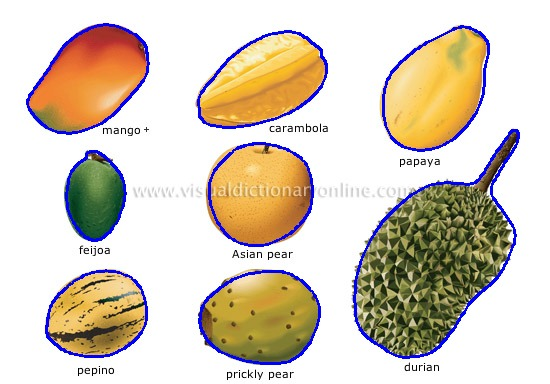
\includegraphics[width=\linewidth]{images/curves.jpg}
\caption[The parametric of listed tropical fruits]{The blue curves are
  the parametric contours of some tropical fruits [\\
  http://visual.merriam-webster.com/images/food-kitchen/food/fruits/tropical-fruits\_4.jpg
  ]}
\label{fig:prior}
\end{figure}

There are two ways to generate control points:
manual initialization and automated initialization. The former is
given as a simple form by hand. % It is easy to use and
% control. However, there are some problems and limitations in case that
% the cost of manual operation is large, or vision deviation due to
% similar brightness between object and background. Therefore,
Sleace the former is rather tedious, two new
intelligent initialization methods are proposed to extract the
contour.
In this thesis, an initial contour estimation method is described and
implemented by employing the well-known SIFT algorithm~\cite{lowe2004distinctive} for
keypoint detection and matching. In Section~\ref{sec:sift_init} it will be discussed in
more detail.

\section{Model Parametrization}
\label{sec:mp}

By applying the (uniform quadratic or cubic) B-spline interpolation to the control points, a new curve
grouped by a sequence of equidistant distributed points is generated
. The B-spline curve is defined in eq.~\ref{eq:paramcurve} and is
composed of a sequence of points $\mathbf{C} = \{C_0, \ldots,
C_{k}\}, k = N_{C-1}$. $N_C$ denotes the number of sample points in the
parametric curve. $N_C$ is significant for the
performance of the CCD algorithm, because its value is directly
proportional to the circumference of the observed object. For a high
resolution image, more sample points should be taken into account.
Hence, there is a trade-off between computational expense and the
accuracy. We recommend to compute the circumference of a given object before
determining $N_C$ and sample more points near spinodals and corners to
capture key features of the object.

Since the resulting parametric curve is continuous and
differentiable, we can compute the normal $\mathbf{n} = \{n_0, \ldots,
n_{k}\}$ and the tangent vector $\mathbf{t} = \{t_0, \ldots, t_{k}\}$
which was discussed in Section~\ref{sec:pbc}. 

In the planar affine shape-space $\mathcal{S}$, the contour, a
hypothetical initial estimate, can be compactly represented using a
vector $\mathbf{\Phi}$ with 6 real elements, namely model
parameters vector. From the perspective of probability, the hypothetical
curve gives a uncertainty, the solution of the curving problem is
therefore no longer just a single curve, but a whole family of
possible curves (Fig.~\ref{fig:prior}). The Gaussian probability density for these possible
curves in shape-space $\mathcal{S}$ is given as:

\begin{equation}
  \label{eq:prior}
   p(\mathbf{\Phi}) \propto
\mathrm{exp} \left\{ -\frac{1}{2} (\mathbf{\Phi} -
  \mathbf{\Sigma}_{\mathbf{\Phi}})^T \mathbf{\Sigma}_{\mathbf{\Phi}}^{-1} (\mathbf{\Phi} -
  \mathbf{\Sigma}_{\mathbf{\Phi}}) \right\}
\end{equation}

\begin{figure}[htb]
  \centering
  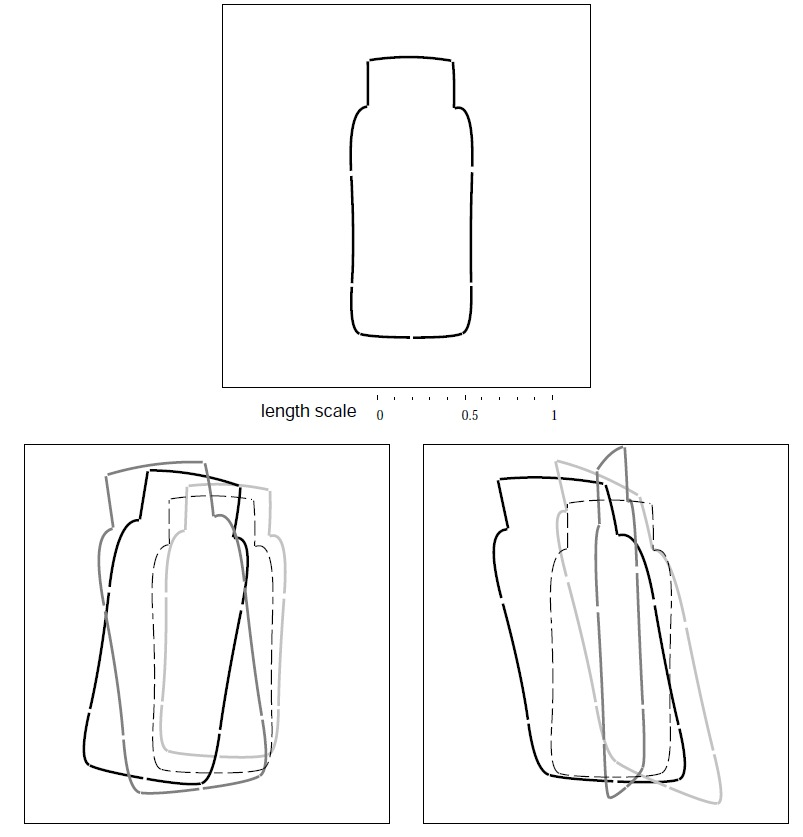
\includegraphics[width=10cm]{images/prior.jpg}
\caption[Sampling from curve families~\cite{blake1998active}]{The top
  figure is the mean shape, the left one represents the euclidean
  similarities, the right one
  sketches some samples in affine space. All these are governed by a
  Gaussian distribution in shape-space with root-mean-square
  displacement of 0.3 length units.}
\label{fig:prior}
\end{figure}

In two dimensions, $\mathbf{\Sigma}_{\mathbf{\Phi}}$ is a $6 \times 6$ 
covariance matrix, which measures the variability of
how much two groups of model parameters change together. The
information matrix $\mathbf{\Sigma}_{\mathbf{\Phi}}^{-1}$ can be
written as 
\begin{equation}
  \label{eq:infomatrix}
  \mathbf{\Sigma}_{\mathbf{\Phi}}^{-1} = \frac{N_{\mathbf{\Phi}}}{\rho_0^2} \mathbf{A}^T\mathcal{U}\mathbf{A}
\end{equation}

where $\rho_0^2$ denotes the mean-square displacement along the entire
curve (\cite{blake1998active}). $\mathbf{A}$ is the shape-matrix, and $\mathcal{U}$ is
metric matrix for curves. $N_{\mathbf{\Phi}}$ represents
the number of model parameters. Note $\rho_0^2$
is a real value and can be computed easily as 
\begin{equation}
  \label{eq:trace}
  \rho_0^2 = \mathrm{tr}(\mathbf{\Sigma}_{\mathbf{\Phi}})
\end{equation}
where $\mathrm{tr}(\cdot)$ operation denotes the trace of a matrix.

The pre-processed input images and the parametric curve model have
thus been set up. In the following sections, the iterative procedure of the
CCD algorithm will be described in detail.

\section{Local statistics}
\label{sec:ls}

\subsection{Collecting local information}
\label{sec:cls}

As claimed in Chapter~\ref{sec:ccdcfp}, one of advantages of the
model-based approach is that we can restrict a task at hand to the ROI
which is
expected to reduce the computational cost. Hence, we first define
the region which contains pixels in the vicinity of the expected image
curve. Considering the complexity and the expense of computing, it is practicable
to choose those pixels actually required for interpolation along
normals of the curve. This is proved useful and important for image
perception and real-time tracking system. In the implementation of
this thesis, the processing is limited to a segment of each normal within
a search region. A fixed distance $h$ along the normal segment is
chosen according to the hypothetical uncertainty of the parametric curve. In the
special case of the norm-squared prior in spline space, a reasonable
search segment is determined as follows:

\begin{equation}
  \label{eq:radius}
  h = \sqrt{2} \rho_0 = \sqrt{\mathrm{tr}(\mathbf{\Sigma}_{\mathbf{\Phi}}\mathbf{A}^T\mathcal{U}\mathbf{A})}
\end{equation}

$h$ denotes the size of a \textit{window} which is used for computing
the local statistics. In the beginning of the iterative procedure, the value
is relatively big and only roughly approximates the vicinity of the image curve
. The
uncertainty is reduced after further iteration steps and as a result, the $h$ becomes smaller and
smaller. After determining the length of the search segment, 
a set of points located on these segments can be collected and
evaluated. Note that the parametric model curve is not required to be
closed, but it shall always encompass a limited area. We only plan to
analyze the pixels located in the vicinity of the contour. Therefore,
we should pay attention to limit the search distance on the
\textit{inner} side in order to avoid crossing the opposite
boundary to sample pixels from the wrong area~\cite{panin2006fully}. In order to
decrease the computational expense, it is advisable to uniformly sample those
pixels on both segments in the vicinity of the contour. On the other
hand, we should avoid to collect too small number of pixels, because
it is statistically invalid and can not
capture all features near the contour. Let us denote the
sample distance using $\delta h$, then the overall number of spaced
sample points $L$ ($2L$ for both sides in all) can be given by:
\begin{equation}
  \label{eq:sample}
  L = \lfloor \frac{h}{\delta h} \rfloor
\end{equation}

Note that the goal of the algorithm is to assign each pixel
($\mathrm{v}_{k,l}, k \in [0,\ldots,N_{\mathrm{C}}-1], l \in [0,
2L-1]$) on either side of the contour. By doing so we thus run into a
classification problem.
Although each pixel should be assigned to one and only
one class so that the target variable is discrete, we can model the
posterior probabilities that lie in $(0,1)$, thus it is similar to a
regression problem. To achieve this, we model the probabilistic
assignments $\mathbf{a}_{v}$ for each pixel $\mathrm{v}_{k,l}$ as following:
\begin{equation}
  \label{eq:pa}
  \mathbf{a}_v  = (a_{v,1}, a_{v,2})^T
\end{equation}
where $a_{v,1}$ describes to which extent a pixel $v$ is expected to
be influenced by side $1$ of the curve, and $a_{v,2}$ is equivalent
for side 2 given by $a_{v,2} = 1- a_{v,1}$. For arbitrary curve
$\mathbf{C}$, it is difficult to give a closed form of $a_v$. In the
following, an efficient approximation of the assignment is derived.

We use the \textbf{signed} distance between pixel
$\mathrm{v}_{k,l}$ and a given curve $\mathbf{C}$ (Fig.~\ref{fig:dis}). $d_{k,l}$
can be approximated by
\begin{equation}
  \label{eq:dis}
  d_{k,l} = \mathbf{n}_k \cdot ( \mathbf{v}_{k,l} - C_k)
\end{equation}

\begin{figure}[htbp]
  \centering
  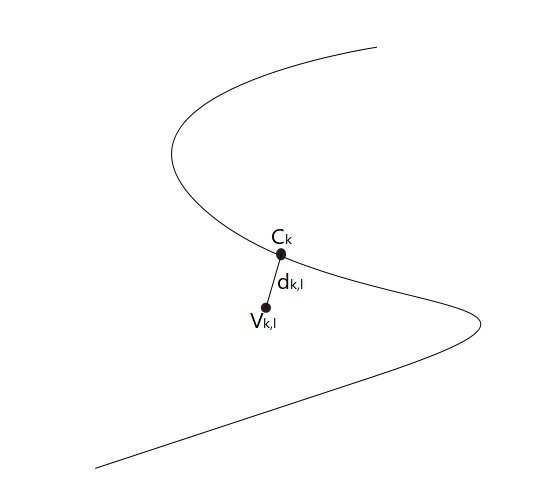
\includegraphics[width=10cm]{images/dis.jpg}
  \caption[The distance between a curve point and a pixel in the vicinity
  of a contour]{The distance between a curve point and a pixel in the
    vicinity of a contour: $C_k$ is the curve point, $v_{k,l}$ is a
    pixel in the perpendicular of the contour, $d_{k,l}$ is the
    distance between $C_k$ and $v_{k,l}$.}
  \label{fig:dis}
\end{figure}

where $\mathbf{v}_{k,l} = {x_{k,l} \choose y_{k,l}}$ is the axis
components of a pixel
$\mathrm{v}_{k,l}$, and $C_k$ is the equivalent for point $C$ on the
curve given by ${x_k \choose y_k}$. Now consider that the curve is
distorted by a Gaussian $p(\mathbf{\Phi})$ which makes the displacement $d_{k,l}$ also Gaussian distributed: $p(d_{k,l}) \sim
\mathcal{N}(d_{k,l}|m_d, \sigma)$, where $m_d$ and $\sigma$ are mean
and covariance of the distribution. Covariance $\sigma$ is expressed as:
\begin{equation}
  \label{eq:cov}
  \sigma = \mathbf{n}_k \cdot \mathbf{J}_k \cdot \mathbf{\Sigma}_{\Phi}
  \cdot \mathbf{J}_k^T \cdot \mathbf{n}_k^T
\end{equation}
where $\mathbf{J}_k$ is the Jacobian of curve $\mathbf{C}$. $\sigma$
can be taken as the uncertainty of the curve along the normal
introduced by the covariance
$\mathbf{\Sigma}_{\mathbf{\Phi}}$, it is a constant and can be
evaluated offline. The variable
$\frac{d_{k,l}}{\sigma}$ now becomes a linear function with respect to $\mathbf{\Phi}$.

In order to apply the probabilistic generative models to the
classification problem,
% calculate the the probability that a point lies on side 1 of the curve
we need to transform the linear function of $\mathbf{\Phi}$ using a
non-linear activation function $f(\cdot)$~\cite{bishop2006pattern} so that 
\begin{equation}
  \label{eq:nonla}
  a_{v,1} = f(\frac{d_{k,l}}{\sigma})
\end{equation}
Currently, two main non-linear activation functions are mostly used
to solve the classification problem. The first is known as the
\textit{logistic sigmoid} function, and is given by
\begin{equation}
  \label{eq:logistic}
  a_{v,1} =
  \frac{1}{1+\mathrm{exp}(\frac{d_{k,l}}{\sqrt{2}\sigma}))}\qquad .
\end{equation}
The term \textit{sigmoid} stands for
S-shaped~\cite{bishop2006pattern}. In~\cite{hanek2004contracting},
another activation function named probit is used, which is defined by
\begin{equation}
  \label{eq:erf}
  a_{v,1} = \frac{1}{2}erf(\frac{d_{k,l}}{\sqrt{2}\sigma} + 1)\qquad ,
\end{equation}
where the error function of a Gaussian distribution is used. Both
two functions in Eq.~\ref{eq:erf} and Eq.~\ref{eq:logistic} are
S-shaped (Fig.~\ref{fig:s-shaped}).
\begin{figure} 
  \begin{minipage}[t]{0.5\linewidth} 
    \centering 
        \subfloat[logistic sigmoid function]{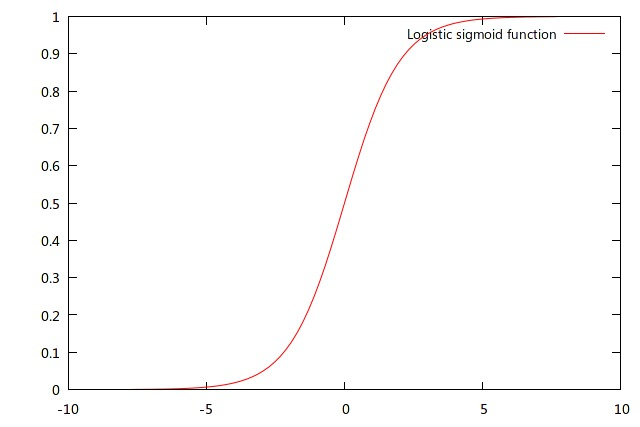
\includegraphics[width=8.0cm]{images/logistic.jpg}}
  \end{minipage}% 
  \begin{minipage}[t]{0.5\linewidth} 
    \centering 
    \subfloat[error function]{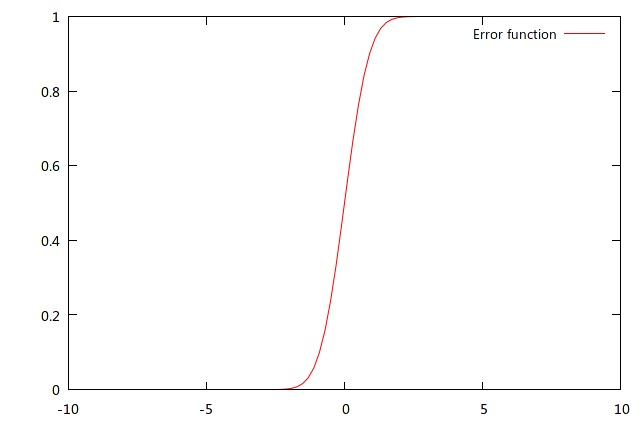
\includegraphics[width=8.0cm]{images/erf.jpg}}
  \end{minipage} 
\caption[Logistic sigmoid function and error function]{Both functions
  are S-shaped}
\label{fig:s-shaped}
\end{figure}

In this thesis, we use both of them to implement the algorithm. They give
similar results but have different behaviors. Logistic sigmoid function
can be perfectly interpreted from the perspective of
possibility. Consider the side $s \in \{0,1\}$, the posterior
distribution for side $s = 1$ can be written as
\begin{eqnarray}
  \label{eq:pdfs}
  p(s=1|I) &=& \frac{p(I|s=1)p(s=1)}{p(I|s=1)p(s=1)
    + p(I|s=2)p(s=2)}\\
&=&  \frac{1}{1+exp(-\mathcal{S})}
\end{eqnarray}
where I is pixels' RGB value, and $\mathcal{S}$ is defined as
\begin{equation}
  \label{eq:ratio}
  \mathcal{S} = \frac{p(I|s=1)p(s=1)}{p(I|s=2)p(s=2)}
\end{equation}
The logistic sigmoid plays an important role in many classification
algorithms. It satisfies the symmetry property, and its inverse 
is known as \textit{logit} function, which represents the log of the
ratio of probabilities $ln [p(s=1|I)/p(s=2|I)]$ for the two classes,
also known as the log odds~\cite{bishop2006pattern}.

The logistic sigmoid function can be used to transform a broad range
of class-conditional distributions, described by the exponential
family, to a non-linear posterior class probabilities. Since not all choices of
class-conditional density are trivial, the probit function is explored
to cope with other complex distributions. The results of logistic
sigmoid function and probit function tend to be similar, except that the
probit function is sensitive to outliers because the logistic sigmoid
decays asymptotically like $\mathrm{exp}(-x)$ for $x \rightarrow \infty$, whereas
for the probit activation function the decay is like $\mathrm{exp}(-x^2)$.

% Generally, we can call this approximation process as \textit{fuzzy} (or \textit{smooth})
% assignment. The accuracy of this assignment will increase as the
% uncertainty of curve governed by covariance $\mathbf{\Sigma}_{\mathrm{\Phi}}$ decreases.

With this assignment and following the suggested rule in~\cite{hanek2004contracting}, we now start to assign two suitable weighting functions
$\omega_1$, $\omega_2$ to the pixels $\mathrm{v}_{k,l}$ along the
normal for the two sides of the curve. the weighting functions are
defined as

\begin{equation}
  \label{eq:weight}
  \omega_{1/2}(d_{k,l}) = C\left(\frac{a_{1/2}(d_{k,l}) -
    \gamma_1}{1-\gamma_2}\right)^4 \left[e^{-d_{k,l}/(2\hat{\sigma}^2)} - e^{-\gamma_2}\right]^+
\end{equation}


where $\gamma_1$ equals to $0.5$ (disjoint weight assignment) and $\gamma_2$
equals to $4$ for the truncated Gaussian~\cite{hanek2004contracting}. 

\begin{figure} 
  \begin{minipage}[t]{0.45\linewidth} 
    \centering 
        \subfloat[]{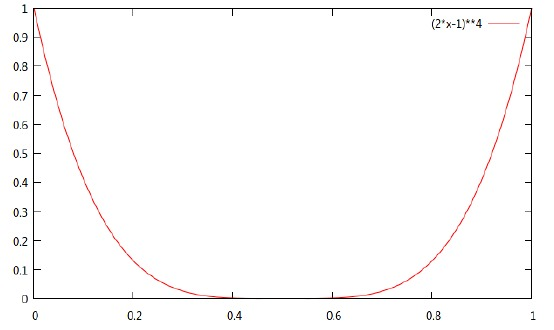
\includegraphics[width=2.0in]{images/weight1.jpg}}
  \end{minipage}% 
  \begin{minipage}[t]{0.45\linewidth} 
    \centering 
    \subfloat[]{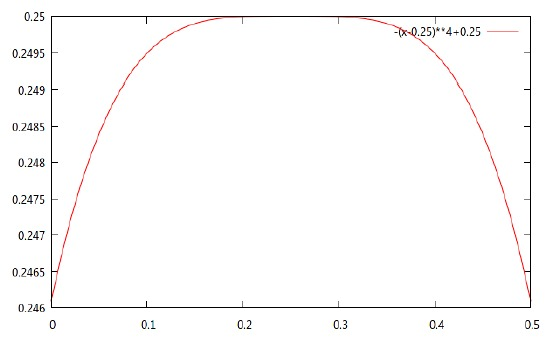
\includegraphics[width=2.0in]{images/weight2.jpg}}
  \end{minipage} 
\caption{the weight functions of the two sides of the contour, a) the
  weight function along the positive direction (outside) in the normal of the
  contour. b) the weight function along the negative direction (inside). }
\label{fig:weight}
\end{figure}

In addition, the standard
deviation is chosen in order to cover the specified distance $h$,
which yields 
\begin{equation}
  \label{eq:deviation}
  \hat{\sigma} = \max \left[\frac{h}{\sqrt(2\gamma_2)}, \gamma_4
  \right], \sigma  = \frac{1}{\gamma_3} \hat{\sigma}
\end{equation}

with the two additional constants $\gamma_3 = 6$ (linear dependence
between $\sigma$ and $\hat{\sigma}$) and $\gamma_4 = 4$ (minimum
weighting window width) as discussed in~\cite{panin2006efficient}. 

In the implementation of this thesis,
all $2 \cdot L \cdot N_C$ distance ($d_{k,l}$), fuzzy assignment
($a_{v,1}(d_{k,l}))$ and weight function ($\omega_1(d_{k,l})$,
$\omega_1(d_{k,l})$) are evaluated offline and saved in an array. Now we have restricted our analysis region of interest in the
limited area, and collected all statistical information required to learn
local statistics. In the next part, we will evaluate the local
statistics.

\subsection{Learning local statistics}
\label{sec:lls}

Given the pixel coordinates and RGB values (For the moment, we only consider raw RGB
statistics), assignment and weight
function, local mean vectors $\mathbf{m}_{v,s}$  and local covariance matrices
$\mathbf{\Sigma}_{\mathbf{\Phi}}$ will be derived for each side $s \in
\{1,2\}$ of the curve.
We first calculate the zero, first and second order weighted moments:
\begin{eqnarray}
  \label{eq:localm}
  M_{k,s}^{(0)}(d_{k,l,s}) &=& \sum_{l=0}^{2L-1} \omega_s(d_{k,l})\\
  \mathbf{M}_{k,s}^{(1)}(d_{k,l,s}) &=& \sum_{l=0}^{2L-1} \omega_s(d_{k,l}) \mathrm{I}_{k,l}\\
  \mathbf{M}_{k,s}^{(2)}(d_{k,l,s}) &=& \sum_{l=0}^{2L-1} \omega_s(d_{k,l}) \mathrm{I}_{k,l}\mathrm{I}_{k,l}^T
\end{eqnarray}

Where $\mathbf{I}$ is just the raw RGB value of a pixel, for a
3-channel image and the values of three components
are  between 0 and 255. The local mean vectors $\mathbf{m}_{v,s}$  and
the local covariance matrices
$\mathbf{\Sigma}_{\mathbf{\Phi}}$  are obtained by
\begin{eqnarray}
  \label{eq:localmean}
  \mathbf{m}_{k,s} &=& \frac{\mathbf{M}^{(1)}_{k,s}}{M^{(0)}_{k,s}}\\
  \label{eq:localcov}
  \mathbf{\Sigma}_{k,s} &=& \frac{\mathbf{M}^{(2)}_{k,s}}{M^{(0)}_{k,s}}
  - \mathbf{m}_{k,s}\mathbf{m}_{k,s}^T  + \kappa \mathbf{I}
\end{eqnarray}
In Eq.~\ref{eq:localcov}, $\kappa I$  means an identity matrix scaled by
$\kappa$ in order to avoid numerical singularity.Later it is namely
required to calculate the inverse matrix of
$\mathbf{\Sigma}_{k,s}$. In our experiments, we choose $\kappa$ to be $\kappa = 0.5$. It is shown that this is efficient to
avoid numerical problems in the process of iteration.

With the local mean vectors $\mathbf{m}_{v,s}$  and the local covariance matrices
$\mathbf{\Sigma}_{\mathbf{\Phi}}$, we can compute the
likelihood function   $p(\mathbf{I}_{k,l} | \mathbf{m}_{v,1}, \mathbf{m}_{v,2},
  \mathbf{\Sigma}_{v,1}, \mathbf{\Sigma}_{v,1})$ for each pixel
  $\mathrm{v}_{k,l}$. In terms of observation model, the likelihood
  function describes how probable the observed data set is for
  different settings of the parameter vector. Hence, we first establish
  the relation between image data $\mathrm{I_{k,l}}$ and the model
  parameter $\mathbf{\Phi}$. Here we model the pixel value
  $\hat{\mathbf{m}}_{k,l}$ and $\hat{\mathbf{\Sigma}}_{k,l}$
  for all pixels $\mathrm{v_{k,l}}$ in the vicinity of the curve as the
  linear combination of $\mathbf{m}_{v,1}$ and $\mathbf{m}_{v,2}$

  \begin{equation}
    \label{eq:meankl}
    \hat{\mathbf{m}}_{k,l} = a_{v,1}(d_{k,l})\mathbf{m}_{v,1} + a_{v,2}(d_{k,l})\mathbf{m}_{v,2}
  \end{equation}

If we define  $\hat{\mathbf{\Sigma}}_{k,l}$ using the rule as
$\hat{\mathbf{m}}_{k,l}$ resulting in a function about $d_{k,l}$, the computational cost in the procedure of
parameters refinement which is discussed in the next section  will be dramatically high. Instead, we decide to
model the covariance matrix $\hat{\mathbf{\Sigma}}_{k,l}$ following the
rule in~\cite{hanek2004fitting}, but we discard this relation:
\begin{equation}
  \label{eq:sigmakl}
  \hat{\mathbf{\mathbf{\Sigma}}}_{k,l} = a_{v,1}(d_{k,l})\mathbf{\Sigma}_{v,1} + a_{v,2}(d_{k,l})\mathbf{\Sigma}_{v,2}
\end{equation}

Now for each observed pixel $\mathbf{I}_{k,l}$, the likelihood
function is given by
\begin{equation}
  \label{eq:likelihood}
p(\mathbf{I}_{k,l} | \mathbf{m}_{v,1}, \mathbf{m}_{v,2},
  \mathbf{\Sigma}_{v,1}, \mathbf{\Sigma}_{v,1}) = p(\mathbf{I}_{k,l} | \hat{\mathbf{\mathbf{m}}}_{k,l},\hat{\mathbf{\mathbf{\Sigma}}}_{k,l}) 
\end{equation}
However, we require the likelihood for all pixels in the vicinity of
the curve. If we consider the coupling or other complex relation among
different group of pixels, the problem will become intractable and the cost of computing will be very expensive. We can
avoid these problems if we assume pixels to be drawn independently from the same distribution
, namely independent and identically distributed
(i.i.d)~\cite{bishop2006pattern}. Thus we can model the likelihood function as
\begin{equation}
  \label{eq:liklihoodall}
  p(\mathbf{I}_{\mathcal{V}} |
  \hat{\mathbf{\mathbf{m}}}_{\mathcal{V}},\hat{\mathbf{\mathbf{\Sigma}}}_{\mathcal{V}})
  = \prod_l \prod_k p(\mathbf{I}_{k,l} | \hat{\mathbf{\mathbf{m}}}_{k,l},\hat{\mathbf{\mathbf{\Sigma}}}_{k,l}) 
\end{equation}

The index $\mathcal{V}$ indicates quantities for all pixels $v$ in
$\mathcal{V}$. Note that we only take into account those pixels which are
in the vicinity $\mathcal{V}$ of the curve, whereas pixels outside
$\mathcal{V}$ are not considered.

Having the likelihood function of observed pixels, as well as
the input data and prior knowledge, now we can go into the parameters
refinement stage to model the conditional distribution.

\section{Refinement of  Parameters}
\label{sec:ref}
In this section, an iterative reweighted least square (IRLS) process is executed to refine parameters,
, model parameter vector and covariance matrix.

With the likelihood function in Eq.\ref{eq:liklihoodall} and prior distribution in
Eq.\ref{eq:prior}, we can model the conditional possibility distribution using:
 % we can estimate the $\hat{\Phi}$ using MAP which is based the
% Bayesian treatment.
% Firstly, the posterior distribution holds
\begin{align}
\label{eq:costf}
    p(\mathbf{\Phi}|\mathbf{\mathbf{I}}_{\mathcal{V}}) 
    \propto &
    p(\mathbf{\mathbf{I}_{\mathcal{V}}}
    |\hat{\mathbf{\mathbf{m}}}_{\mathcal{V}}(\mathrm{\Phi}),\hat{\mathbf{\mathbf{\Sigma}}}_{\mathcal{V}}(\mathrm{\Phi}))p(\mathbf{\Phi}
    | \mathbf{m}_{\mathbf{\Phi}},
    \mathbf{\mathbf{\Sigma}}_{\mathbf{\Phi}})\nonumber\\
    = & {\frac{1}{{(2\pi)}^{1/2}}}
      \frac{1}{|\mathbf{\Sigma}_{\mathbf{\Phi}}|}
      \mathrm{exp}\{-\frac{1}{2}{(\phi-m_{\mathbf{\Phi}})^T{\mathbf{\Sigma}_{\mathbf{\Phi}}}^{-1}(\phi-\mathbf{m}_{\mathbf{\Phi}})}\}\cdot
    \nonumber\\ 
    & \prod_{k = 0}^{N_{C}-1} \prod_{l=0}^{2L-1}{\frac{1}{(2\pi)^{1/2}}
        \frac{1}{|\hat{\mathbf{\Sigma}}_{k,l}|} \mathrm{exp}\{-\frac{1}{2}
        {\left[I_{k,l}-\hat{\mathbf{m}}_{k,l}(a_{v,1})\right]^T\hat{\mathbf{\Sigma}}_{k,l}^{-1}\left[I_{k,l}-\hat{\mathbf{m}}_{k,l}(a_{v,1})\right]}
      }\}
\end{align}
The difference between this conditional distribution and posterior
distribution is that here the former function has not been normalized yet.
If applying logarithm operation to the conditional possibility
distribution, we can define a common cost function $\mathcal{Q}$,
which is given by:
\begin{align}
  \label{eq:costd}
  \mathcal{Q} = & -2 \ln \left\{  p(\mathbf{\mathbf{I}_{\mathcal{V}}}
    |\hat{\mathbf{\mathbf{m}}}_{\mathcal{V}}(\mathrm{\Phi}),\hat{\mathbf{\mathbf{\Sigma}}}_{\mathcal{V}}(\mathrm{\Phi}))p(\mathbf{\Phi}
    | \mathbf{m}_{\mathbf{\Phi}},
    \mathbf{\mathbf{\Sigma}}_{\mathbf{\Phi}})\right\}\nonumber\\
 = & \ln{(2\pi)} + 2\ln{|\mathbf{\Sigma}_{\mathbf{\Phi}}|} +
 {\mathbf{\Phi}}^T{\mathbf{\Sigma}_{\mathbf{\Phi}}}^{-1}\mathbf{\Phi}
 + 2LN_{C} \cdot \ln{2\pi} + \nonumber \\
& 2\sum_{k = 0}^{N_{C}-1} \sum_{l=0}^{2L-1}{\ln{|\mathbf{\Sigma}_{k,l}|}} + \sum_{k = 0}^{N_{C}-1} \sum_{l=0}^{2L-1}
\left\{{\left[I_{k,l}-\hat{\mathbf{m}}_{k,l}(a_{v,1})\right]^T\hat{\mathbf{\Sigma}}_{k,l}^{-1}\left[I_{k,l}-\hat{\mathbf{m}}_{k,l}(a_{v,1})\right]}\right\}
\end{align}

We interpret the estimate $\hat{\mathbf{\Phi}}$ of the model
parameters $\mathbf{\Phi}$ as  the mean $\mathbf{m}_{\mathbf{\Phi}}$ of a Gaussian
approximation of the posterior distribution, and
$\hat{\mathbf{\Phi}}$ can be evaluated as:
\begin{equation}
  \label{eq:maxcost}
  \hat{\mathbf{\Phi}} =
  \mathbf{m}_{\mathbf{\Phi}}\underset{\mathbf{\Phi}}{\arg\max} \
  (\mathcal{Q}) \qquad.
\end{equation}

To optimize $\mathcal{Q}$ based on the estimated $m_{\mathbf{\Phi}}$,
the approximation to the Hessian matrix can be adopted. First we
compute the partial derivatives of $\mathcal{Q}$:

\begin{equation}
\label{eq:partcost}
\nabla_{\mathbf{\Phi}}\{{\mathcal{Q}(\mathbf{\Phi})}\} =  2\{{\mathbf{\Sigma}_{\mathbf{\Phi}}}^{-1}\}^{T}{\mathbf{\Phi}} - \sum_{k = 0}^{N_{C}-1} \sum_{l=0}^{2L-1}
\left\{\mathcal{J}_{a_{v,1}}^T\hat{\mathbf{\Sigma}}_{k,l}^{-1}\left[I_{k,l}-\hat{\mathbf{m}}_{k,l}(a_{v,1})\right]\right\}
\end{equation}

with being:
\begin{equation}
  \label{eq:jocob}
  \mathcal{J}_{a_{v,1}} = \left( \mathbf{m}_{k,1} -\mathbf{m}_{k,2} \right)(\nabla_{\phi} a_{v,1}(d_{k,l}))^T
\end{equation}

and where $a_{v,1}(d_{k,l})$ equals
\begin{equation}
  \label{eq:nablaa}
\nabla_{\mathbf{\Phi}} a_{v,1}(d_{k,l}) = \frac{\partial a_{v,1}(d_{k,l})}{\partial d_{k,l}}
\left( \frac{\partial d_{k,l}}{\partial x_{k,l}}\mathbf{J}_{\mathbf{\Phi}}(\mathrm{v}_{k,l}(x)) + \frac{\partial d_{k,l}}{\partial y_{k,l}}\mathbf{J}_{\mathbf{\Phi}}(\mathrm{v}_{k,l}(y))
 \right)  
\end{equation}
Where $\mathrm{v}_{k,l}(x)$ and $\mathrm{v}_{k,l}(y)$ are the axis
components of pixel $\mathrm{v}_{k,l}$, and $d_{k,l}$ is given by
\begin{equation}
  \label{eq:diskl}
  d_{k,l} = (x_{k,l} - x_{k})n_{k}(x) +(y_{k,l} - y_{k}) n_{k}(y)
\end{equation}
with $n_{k}(x)$ and $n_{k}(y)$ being the components of the normal vector of
curve point $C_{k}$. Moreover, we have
\begin{equation}
  \label{eq:nabladkl}
  \nabla_{\mathbf{\Phi}} a_{v,1}(d_{k,l}) = \frac{1}{\sqrt{2\pi}\sigma} \mathrm{exp}\left\{ -\frac{d_{k,l}^2}{2\sigma^2} \right\}
\left( n_k(x)\mathbf{J}_{\mathbf{\Phi}}(\mathrm{v}_{k,l}(x)) + n_k(y)\mathbf{J}_{\mathbf{\Phi}}(\mathrm{v}_{k,l}(y))
 \right) 
\end{equation}
In terms of the properties of  B-spline curve  and planar affine
model-space. The pixel coordinate of $\mathrm{v}_{kl}$ can be written
as
\begin{eqnarray}
  \label{eq:vkl}
\mathrm{v}_{k,l}(x) &= & \mathbf{U}_k^{T}\mathbf{A}_x \mathbf{\Phi} + \mathbf{U}_k P_0(x) + \Delta_h n_k(x) \\
          &=&\Phi_0\sum_{i}^nU_{k,i} +
          (1+\Phi_2)\sum_{i}^nU_{k,i}*x_{k,i} + \Phi_{5}\sum_{i}^n
          U_{k,i}y_{k,i} + \Delta_h n_k(x)\\
\mathrm{v}_{k,l}(y) &=& \mathbf{U}_k^{T}\mathbf{A}_y \mathbf{\Phi} +
\mathbf{U}_k P_0(y) + \Delta_h n_k(y) \\
          &=&\Phi_1\sum_{i}^nU_{k,i} +
          (1+\Phi_3)\sum_{i}^nU_{k,i}*y_{k,i} + \Phi_{4}\sum_{i}^n
          U_{k,i}x_{k,i} + \Delta_h n_k(y)
\end{eqnarray}

Now we can compute $\mathbf{J}_{\mathbf{\Phi}}$ as follows:

\begin{equation}
  \label{eq:bigj}
\mathbf{J}_{\mathbf{\Phi}}(\mathrm{v}_{k,l}) =
\left[ {\begin{array}{cccccc}
\frac{\partial \mathrm{v}_{k,l}(x)}{\partial \Phi_0}& \frac{\partial \mathrm{v}_{k,l}(x)}{\partial \Phi_1}& \frac{\partial \mathrm{v}_{k,l}(x)}{\partial \Phi_2}& \frac{\partial \mathrm{v}_{k,l}(x)}{\partial \Phi_3}&\frac{\partial \mathrm{v}_{k,l}(x)}{\partial \Phi_4} &\frac{\partial \mathrm{v}_{k,l}(x)}{\partial \Phi_5}  \\
\frac{\partial \mathrm{v}_{k,l}(y)}{\partial \Phi_0}& \frac{\partial \mathrm{v}_{k,l}(y)}{\partial \Phi_1}& \frac{\partial \mathrm{v}_{k,l}(y)}{\partial \Phi_2}& \frac{\partial \mathrm{v}_{k,l}(y)}{\partial \Phi_3}&\frac{\partial \mathrm{v}_{k,l}(y)}{\partial \Phi_4} &\frac{\partial \mathrm{v}_{k,l}(y)}{\partial \Phi_5}  \\
 \end{array} } \right]
\end{equation}

Afterwords, the Gauss-Newton approximation to the Hessian
matrix is given by

\begin{equation}
  \label{eq:hessian}
  \mathcal{H}_{\mathbf{\Phi}} \mathcal{Q}  =
  \mathbf{\Sigma}_{\mathbf{\Phi}}^{-1} + \sum_{k = 0}^{N_{C}-1}
  \sum_{l=0}^{2L-1} \left\{\mathcal{J}_{a_{v,1}}^T\hat{\mathbf{\Sigma}}_{k,l}^{-1}\mathcal{J}_{a_{v,1}}\right\}\qquad.
\end{equation}


The overall gradient and Hessian matrices for the optimization
are obtained by adding the prior cost function
derivatives, and the Newton optimization step can finally be
performed as

\begin{eqnarray}
\label{eq:newton}
  \mathbf{m}_{\mathbf{\Phi}}^{new} & = &
  \mathbf{m}_{\mathbf{\Phi}} - (\mathcal{H}_{\mathbf{\Phi}}
  \mathcal{Q})^{-1} \nabla_{\mathbf{\Phi}} \mathcal{Q} \nonumber \\
  \mathbf{\Sigma}_{\mathbf{\Phi}}^{new} & = &
  c\mathbf{\Sigma}_{\mathbf{\Phi}} - (1-c)(\mathcal{H}_{\mathbf{\Phi}}
  \mathcal{Q})^{-1}
\end{eqnarray}
with $c$ empirically set to $\frac{1}{4}$. Note that the covariance
matrix is updated by an exponential decay rule as well. Coefficient $c$ specifies the
maximum decrease of the covariance within one iteration
step~\cite{hanek2004contracting}. If $c$ is very large, due to the slow reduction of covariance the
convergence process will be very slow. On one hand if $c$ is
very small, CCD might diverge.

We can investigate the iteration process of the CCD algorithm by
comparing it to the counterpart of K-means or EM algorithms, both of
which also include two stages. First it is required to choose some
initial values for the parameters governing the posterior
distribution. Then in the E (expectation) step, a cost function is
being minimized while keeping the parameters fixed. In the M (maximization)
step, calculation of the new values is being done while keeping the
expectation values fixed. This two-stage optimization is then repeated
until convergence. 

% In the beginning of iteration, due to the accuracy of the
% estimate of $\mathbf{m}_{\mathbf{\Phi}}$ and
% $\mathbf{\Sigma}_{\mathbf{\Phi}}$. 

The two stages of the CCD algorithm are iterated until the convergence
criterion is satisfied. After each iteration step, there are two
model parameters vectors $\mathbf{m}_{\mathbf{\Phi}}^{old}$ and
$\mathbf{m}_{\mathbf{\Phi}}^{\mathrm{new}}$, which correspond to the
spline curves $\mathbf{C}^{\mathrm{old}}$ and
$\mathbf{C}^{\mathrm{new}}$ respectively. Which kind of convergence
criterion should we choose? Two choices, one is using the norm of
difference between $\mathbf{m}_{\mathbf{\Phi}}^{old}$ and
$\mathbf{m}_{\mathbf{\Phi}}^{\mathrm{new}}$, another is measuring
the displacement between two spline curves, $\mathbf{C}^{\mathrm{old}}$ and
$\mathbf{C}^{\mathrm{new}}$. Experiments show that the measure of
curve difference using the norm is sensitive to parametrization, and
computation of the normal curve-displacement measure $D(\mathbf{C}^{new},
\mathbf{C}^{old})$  is feasible if we are content with
local, rather than global minimization. The normal curve-displacement
between two points on $\mathbf{C}^{new}(u)$ and $\mathbf{C}^{old}(u)$ is given by:
\begin{equation}
  \label{eq:normald}
  D(u) \approx
  [C^{new}(u) - C^{old}(u)] \cdot \mathbf{n}(u)\qquad.
\end{equation}

The total displacement $C^{new}(u) - C^{old}(u)$
 at a point represents the sum of components along
the curve tangent and normal respectively. The tangential component
approximates the displacement along the curve
$\mathbf{C}^{old}$, which reflects the variation of parameterisation
between curves. If the tangential component is eliminated, the normal
component will represent purely the distance between curves~\cite{blake1998active}. The
use of normal displacement is a standard technique in the field of computer vision
and can be explained intuitively. 
Traversing all points on curves, the curve-displacement equals to:
\begin{equation}
  \label{eq:bigD}
  D(\mathbf{C}^{new}, \mathbf{C}^{old})  = \sum_{i=0}^{N_{C}-1} [C_{i}^{new} - C_{i}^{old})] \cdot \mathbf{n}_{i}
\end{equation}
In the implementation of this thesis, we use the $\mathbf{C}^{new} -
\mathbf{C}^{old})$ as the convergence criterion of the
iteration. Moreover, the curve-displacement can also be used to detect
and delete outliers~\cite{blake1998active}.

Finally, the best recorded estimate
$\mathbf{m}_{\mathbf{\Phi}}^{best}$ and
$\mathbf{\Sigma}_{\mathbf{\Phi}}^{best}$ will be given as output of the
CCD algorithm.


\section{The CCD Tracker}
\label{sec:vg}

We have devised the CCD algorithm in the previous section. Generally,
it is used to cope with the curve-fitting problem in a single
image. Like some other model-based segmentation algorithms, the CCD
algorithm can also be used to handle object tracking problem in a
sequence of images captured at successive time-steps. % Some
% distinguishing characteristics of make it stable and efficient.

In this section we describe a naive tracking algorithm based on the CCD
algorithm.

A sequence of image for example, video data, consist of neighboring 2-D slices of a
higher-dimensional volume. Usually two neighboring frames have similar
information and features and might only be distinguished by
investigating in detail. Hence, a naive CCD tracking algorithm can be
 be obtained by applying the CCD algorithm to each frame
 independently, and the output of parameters obtained from  the
 previous frame can be used in the next frame. However, such
 a tracker would be of limited use because the expense of computation
 will be intolerable in a practical environment which requires high
 performance and efficiency. Furthermore, without exploiting
 statistical dependencies between successive images, the tracker can
 not work if a radical change or big perturbation happened while
 switching into a new frame. A real-time CCD tracker exploiting the
 coherence of curve motion and the temporal coherence of pixel values
 is proposed in~\cite{hanek2004fitting}. 


\section{Summary of the CCD algorithm and its variant}
\label{sec:sccd}
In this section,  for sake of clarity, a sketch of the naive CCD
tracker is given below. Note that we only consider the manual
implementation.  
% \newcommand{\redvline}{\color{red} \vrule width 4pt}
\begin{table}[htbp]
  \caption{Algorithm: the naive Contracting Curve Density (CCD) tracker}
  \label{summary of CCD}
  \centering
  \begin{tabular*}{0.9\textwidth}{!{\color{red} \vrule width 4pt}l}
\textbf{Input}:\parbox{13cm}{ 
  \begin{enumerate}
  \item Sequence image data $\mathbf{I}(t)$, $t$ denotes the time-step
  \item A set of control points:  $\mathbf{P} = \{P_{0}, \ldots, P_{N_{cp}}\}$,
$N_{cp}$ is the number of control points.
  \end{enumerate}
}
\\
\textbf{Output}: 
\parbox{13cm}{
  \begin{enumerate}
  \item Estimate model parameter vector $\mathbf{m}_{\mathbf{\Phi}}^{best}$ 
  \item Corresponding covariance matrix $\mathbf{\Sigma}_{\mathbf{\Phi}}^{best}$
  \end{enumerate}
}
\\
\textbf{Initialization}:\parbox{13cm}
{
  \begin{enumerate}
  \item Apply some pre-processing methods to the image data to
    $\mathbf{I}(0)$, $0$ denotes the first frame
  \item Compute the B-spline curve $\mathbf{C}_{0}(u)$ and
    corresponding normal and tangent vectors 
  \item Initialize $\mathbf{\Sigma}_{\mathbf{\Phi}}(0)$ as zero vector
  \item Compute the $\mathbf{\Sigma}_{\mathbf{\Phi}}(0)$
  \end{enumerate}
}\\
\textbf{Main loop}: 
\parbox{13cm}
{
If the time-step $t > 0$, execute the \textit{initialization} step for
the frame of image. Firstly do pre-processing, then initialize $\mathbf{\Sigma}_{\mathbf{\Phi}}(t)$ as
$\mathbf{\Sigma}_{\mathbf{\Phi}}^{best}(t-1)$, and generate a new
B-spline curve using $\mathbf{\Sigma}_{\mathbf{\Phi}}(t)$,
last compute the $\mathbf{\Sigma}_{\mathbf{\Phi}}(0)$. After these
initialization steps, go into loop of  two stages of the CCD algorithm.
}\\

\parbox{2cm}{$\quad$}\parbox{13cm}
{
  \begin{enumerate}
  \item Compute the uncertainty norm, segment length $h$ in terms of
    current estimate
  \item Collect the pixels $\mathrm{v}_{k,l}$ according to the $h$ and
    assign weights to these pixels.
  \item Compute the local statistics $\mathbf{m}_{k,s}$ and $\mathbf{\Sigma}_{k,s}$
  \item Evaluated the observed model parameters
    $\hat{\mathbf{m}}_{k,l}$ and $\hat{\mathbf{\Sigma}}_{k,l}$
  \item Compute the gradient $\nabla_{\mathbf{\Phi}}\mathcal{Q}$ and the Hessian $\mathcal{H}_{\mathbf{\Phi}}\mathcal{Q}$
  \item Apply optimization algorithm to the  $\mathcal{Q}$ in order to
    to compute the $\mathbf{m}_{\mathbf{\Phi}}^{new}$ and $\mathbf{\Sigma}_{\mathbf{\Phi}}^{new}$
  \item Compute the curve-displacement $\mathbf{D}(\mathbf{C}^{new},
    \mathbf{C}^{old})$, if it is satisfied with the convergence
    criterion, accept the $\mathbf{m}_{\mathbf{\Phi}}^{best}(t)$ and
    $\mathbf{\Sigma}_{\mathbf{\Phi}}^{best}$. Otherwise, go to step 1
    and until convergence.
  \end{enumerate}
}
\\
\parbox{2cm}{$\quad$}\parbox{13cm}
{
Ff convergence condition is satisfied,
$\mathbf{m}_{\mathbf{\Phi}}^{best}(t)$ and
$\mathbf{\Phi}_{\mathbf{\Phi}}^{best}(t)$ are obtained. Then read a
new frame of an image and go to the beginning of main loop.
}
  \end{tabular*}
\end{table}
\section{Efficiency and complexity}
\label{sec:eff}
In this section, we discuss the complexity of the CCD algorithm. 
The time complexity of calculating the local statistics is
$\mathcal{O}(N_{C}\times L)$, where $N_{C}$ is the number of sampled
points along the contour, $2L$ is the number of pixels in the vicinity
of the contour. The time consumed for Gaussian-Newton method is still
$\mathcal{O}(N_{C}\times L)$. Because of the special structure used to
calculate the local statistics, the runtime only increases with the
scale of observed object in an image, and experiments show that the algorithm
works well even when keeping small number of points along the contour for
high resolution images, and in the process, runtime does not increase.

